% -*- root: ../EstadisticaII.tex -*-

\chapter{Regresión}
El objetivo de la regresión es predecir una/s variable/s en función de la/s otra/s.


\section{Regresión lineal}

Observamos dos variables, X e Y , el objetivo es analizar la relación existente entre ambas, de forma que podamos predecir o aproximar el valor de la variable Y a partir del valor de la variable X.

\begin{itemize}
\item La variable Y se llama variable respuesta.
\item La variable X se llama variable regresora o explicativa.
\end{itemize}

Por ejemplo:
\begin{center}
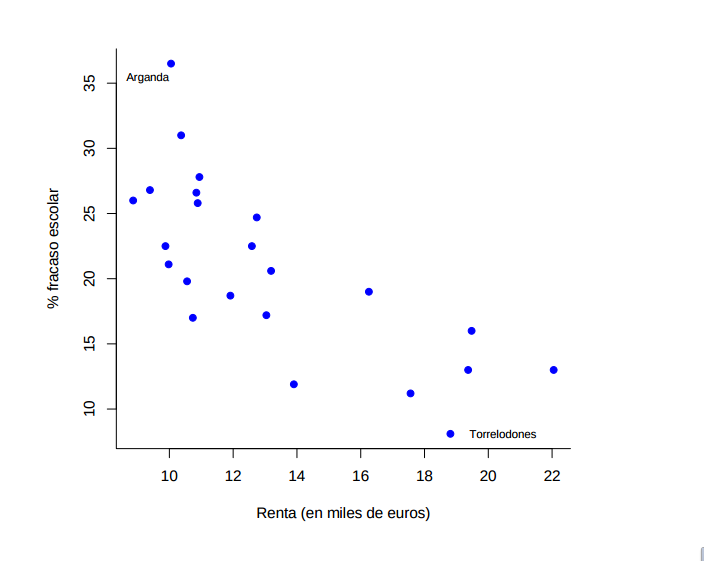
\includegraphics[scale=0.5]{img/RentaVsFracaso.png}
\end{center}

Queremos predecir el fracaso escolar en función de la renta. La variable respuesta es el fracaso escolar, mientras que la variable regresora es la renta.

\subsection{Regresión lineal simple}

Frecuentemente existe una relación lineal entre las variables. En el caso del fracaso escolar,queremos construir una recta $Y_i = β_0 X_i + β_1\; i=1,...,n$ que minimice el error.

El problema es estimar los parámetros $β_0,β_1$. Una manera de hacer esto es:

\subsubsection{Recta de mínimos cuadrados}

\begin{defn}[Recta de mínimos cuadrados]
Estimando $β_i$ por $\hat{β_i}$ obtenemos: \[\hat{Y_i} = \hat{β}_0 + \hat{β}_1 x_i\]

La recta viene dada por los valores $\hat{β_0}, \hat{β_1}$ para los que se minimiza el error cuadrático, es decir:
\[\sum_{i=1}^n \left(Y_i - \hat{Y_i}\right)^2 =  \sum_{i=1}^n \left[ Y_i - (\hat{β_0} + \hat{β_1}x_i) \right]^2\]
\end{defn}

\begin{example}
\begin{center}
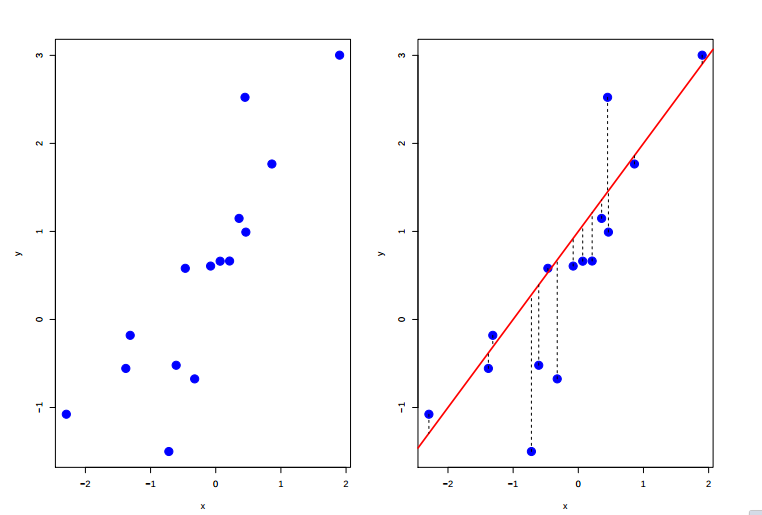
\includegraphics[scale = 0.6]{img/ejemploRectaRegresionLineal.png}
\end{center}
\end{example}

\paragraph{Cómo calcular la pendiente} de la recta de mínimos cuadrados.


Vamos a ver unas pocas maneras de calcular la recta de mínimos cuadrados.

\begin{itemize}

	\item El sistema habitual:

	\[ \hat{β_1} = \frac{\sum_{i=1}^n(x_i - \bar{x})(Y_i - \bar{Y})}{\sum_{i=1}^n (x_i - \bar{x})^2} = \frac{S_{xy}}{S_{xx}} \]
	Donde
		\[S_{xy} = \sum_{i=1}^n(x_i - \bar{x})(Y_i - \bar{Y}) \]
		\label{Ssubxx}
		Y, consecuentemente, como el avispado lector podrá imaginar
		\[S_{xx} = \sum_{i=1}^n (x_i - \bar{x})^2\]

		Es interesante darse cuenta que, siendo $S_x$ la cuasivarianza, tenemos $S_{xx} = (n-1)S_x$


	\subitem \[β_0 = \bar{Y} - \hat{β_1}\bar{x}\]

	\textbf{Entonces:}
	\[\text{recta} \equiv y - \bar{y} = \frac{S_{xy}}{S_{xx}}(x - \bar{x} ) \]

	\item Mínimos cuadrados como promedio de pendientes:
	\label{rmc::promediopendientes}
	\[
	\hat{β_1} = \frac{S_{xy}}{S_{xx}} = \sum_{i=1}^n \frac{(x_i - \bar{x})^2}{S_{xx}} \left( \frac{(Y_i - \bar{Y})}{x_i - \bar{x}} \right) = \sum_{i=1}^n ω_i \left( \frac{(Y_i - \bar{Y})}{x_i - \bar{x}} \right)
	\]

	Vemos que hemos ponderado la pendiente de cada recta que une cada punto con la media. Este peso es mayor cuanto mayor es la distancia \textbf{horizontal}.

	\item Mínimos cuadrados como promedio de respuestas:

	\[
	\hat{β_1} = \frac{\sum_{i=1}^n  (x_i - \bar{x}) (Y_i - \bar{Y})}{S_{xx}} \overset{(1)}{=} \sum_{i=1}^n \frac{x_i-\gor{x}}{S_{xx}} Y_i = \sum α_i Y_i
	\]

	$(1) \impliedby$ hemos utilizado una propiedad básica, importantísima y, a simple vista, poco (o nada) intuitiva:

	\begin{prop}
	Sea $\{x_i\},\{y_i\}$ datos de variables aleatorias.
	\[
		\sum (x_i - \gor{x}) (y_i -\gor{y}) = \sum(x_i -\gor{x})y_i = \sum (y_i - \gor{y})x_i
	\]

	\textbf{Importante:} sólo quitamos la media de una de las 2. No podemos hacer $\sum (x_i - \gor{x}) (y_i -\gor{y}) = \sum x_iy_i$, porque esto ya no es verdad.
	\end{prop}
	\begin{proof}
		\[\sum_{i=1}^n (x_i - \gor{x}) (y_i -\gor{y}) = \sum_{i=1}^n (x_i -\gor{x})y_i - \underbrace{\sum_{i=1}^n (x_i-\gor{x})\gor{y}}_{0}\]

		Vamos a ver por qué ese término es 0.
	\[\sum_{i=1}^n (x_i-\gor{x})\gor{y} \overset{(1)}{=} \left(\left(\sum_{i=1}^n x_i\right) - n\gor{x}\right)\frac{\sum y_i}{n}\]

	$(1)\to$ Estamos restando $n$ veces el  término $\gor{x}$ que no tiene índice del sumatorio, con lo que podemos sacarlo fuera.


	Aplicando la propiedad distributiva con el factor $\frac{1}{n}$, obtenemos:


	\[
		\left(\frac{\left(\sum x_i\right)}{n} - \frac{n\gor{x}}{n}\right)\sum_{i=1}^n y_i = (\gor{x} - \gor{x}) \sum y_i = 0
	\]

	\obs Pero... ¿y porqué $\sum(x_i -\gor{x})y_i ≠ 0$? ¿Cuál es el fallo de lo siguiente?

	\[
		\sum(x_i -\gor{x})y_i = \frac{\sum(x_i -\gor{x})y_i}{n}·n
	\]
	¿Y aplicamos el mismo razonamiento que antes?

	La respuesta es que, en este caso el factor $(x_i-\gor{x})$ está multiplicado por $y_i$ \textbf{dentro} del sumatorio, es decir:

	\[
	\sum_{i=1}^n (x_i - \gor{x}) (y_i -\gor{y}) = \sum_{i=1}^n \left[(x_i -\gor{x})y_i\right] - \sum_{i=1}^n \left[(x_i-\gor{x})\gor{y}\right] \]
	Y podemos sacar $\gor{y}$ del sumatorio, porque está multiplicando y no tiene índice del sumatorio.

	\[ \sum_{i=1}^n \left[(x_i -\gor{x})y_i\right] - \sum_{i=1}^n \left[(x_i-\gor{x})\right]\gor{y}
	\]
	\end{proof}

	\begin{prop}Propiedades de estos $α_i$

		\begin{enumerate}
			\item $\sum α_i = 0$
				\begin{proof}
					\[\sum α_i = \sum \frac{(x_i-\gor{x})}{S_{xx}} = 0 \impliedby \sum (x_i-\gor{x}) = 0\]
					\[\sum (x_i-\gor{x}) = \left(\sum x_i\right) - n\gor{x} = \left(\sum x_i\right) - n \frac{\sum x_i}{n} = 0\]
				\end{proof}
			\item $\sum α_ix_i = 1$
				\begin{proof}
					\[ \sum α_ix_i = \sum\frac{(x_i-\gor{x})x_i}{S_{xx}} = \frac{1}{S_{xx}}\sum (x_i-\gor{x})(x_i-\gor{x}) = \frac{S_{xx}}{S_{xx}} = 1\]
				\end{proof}
			\item $\sum α_i^2 = \frac{1}{S_{xx}}$
				\begin{proof}
					\[\sum α_i^2 = \sum \frac{(x_i-\gor{x})(x_i-\gor{x})}{S_{xx}^2} = \sum \frac{(x_i-\gor{x})x_i}{S_{xx}^2} = \sum \frac{α_i x_i}{S_{xx}} = \frac{1}{S_{xx}} \sum α_ix_i \]
					Utilizando el anterior, tenemos $\sum α_i^2= \frac{1}{S_{xx}}$
				\end{proof}

		\end{enumerate}

	\end{prop}


\begin{defn}[Residuo]
En una recta de mínimos cuadrados: Sea $y_i = β_1x_i - β_0$ y sea $\hat{y}_i = \hat{β}_1x_i - \hat{β}_0$, llamamos residuo a $$e_i = y_i - \hat{y}_i$$

Los residuos cumplen:

\[
\sum_{i=1}^n e_i = 0
\]

Esto es intuitivo, ya que los errores se compensan y además es una buena propiedad.
\end{defn}



\begin{prop}
Sean $\{e_i\}$ una variable aleatoria que cumple \footnote{Se ha utilizado la $e$ porque es útil en cuanto a los residuos de la recta de mínimos cuadrados}:
\[\sum e_i = 0\]

Entonces:
\[\sum e_i x_i = 0 \implies \cov{e,x} = 0\]
\end{prop}

\begin{proof}
\[
\cov{e,x} = \esp{e}\esp{x} - \esp{e·x}
\]

Vamos a ver que los 2 sumandos son 0.

 $\esp{e}\esp{x} = 0 \impliedby \esp{e} \overset{?}{=} \gor{e} = 0$


Por otro lado:
\[ \sum (e_i - \vec{µ}) x_i = \sum (e_i - \vec{µ}) (x_i - \vx) \]


\[
\esp{e·x} = \sum e_ix_i = \sum e_ix_i - \vx \sum e_i = \sum e_i(x_i - \vx)
\]
\end{proof}


Esto tiene la siguiente explicación ``intuitiva'': La recta de mínimos cuadrados contiene toda la información lineal que $X$ puede dar sobre $Y$ (debido a que la covarianza entre los residuos y $X$ es 0).
\end{itemize}

\subsubsection{Fallos de la recta de mínimos cuadrados}

Vamos a ver un par de ejemplos ilustrativos:

\begin{example}[Sobre los datos atípicos]

Esta es una recta de mínimos cuadrados calculada para una nube de puntos a la que se ha añadido un punto atípico. Se ve una cierta tendencia de que la pendiente debería ser positiva, pero el dato atípico provoca un cambio brusco.
\begin{center}
%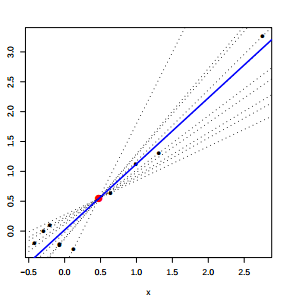
\includegraphics[scale=0.9]{img/rmc_atipico1.png}
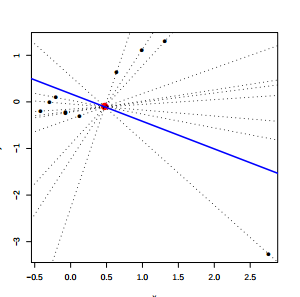
\includegraphics[scale=0.9]{img/rmc_atipico2.png}
\end{center}

\end{example}

\begin{example}[Sobre la distancia horizontal]

¿Y da igual lo atípico que sea un dato? La respuesta es que no. Si el dato es muy atípico en la variable respuesta ($Y$), pero es muy \textit{típico} en la variable regresora, la recta no se desvía tanto. Vamos a verlo y después explicamos la razón.

Esta es la recta, en la que hemos ignorado los 3 datos que parecen ``atípicos''.
\begin{center}
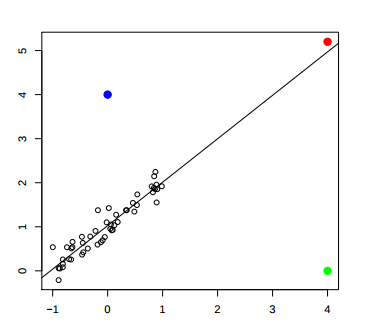
\includegraphics[scale=0.9]{img/sobredistanciahorizontal.png}
\end{center}

Ahora calculamos las rectas teniendo en cuenta sólo uno de los puntos.

\begin{center}
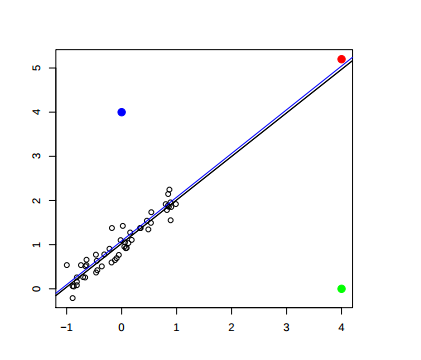
\includegraphics[scale=0.4]{img/sobredistanciahorizontal1.png}
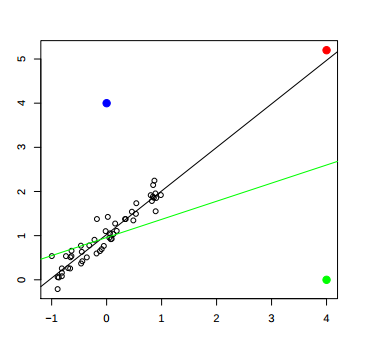
\includegraphics[scale=0.4]{img/sobredistanciahorizontal2.png}
\end{center}

Vemos que la recta azul no se desvía apenas de la original, mientras que la recta verde si se desvía un montón. ¿Esto a qué se debe? A que importa más la distancia horizontal de la media que la distancia vertical. Si vamos a la expresión de la recta de mínimos cuadrados como promedio de las pendientes \label{rmc::promediopendientes} vemos que hay un término $\frac{(x_i - \gor{x})}{S_{xx}}$ que hemos tomado como pesos para ponderar y en este caso, la distancia horizontal $(x_i - \gor{x})$ está multiplicando en el numerador.



\end{example}





\subsubsection{Introduciendo ``aleatoreidad'' para poder hacer IC}

Sea $\{ε_i\}$ siendo $ε_i \sim N(0,σ^2)$. Lo habitual es no saber cómo han sido generados los datos y es probable que no vayamos a conocer con exactitud absoluta la recta de mínimos cuadrados. Es por ello que suponemos el siguiente modelo para la variable respuesta:

\[
Y_i = β_1 x_i + β_0 + ε_i
\]


Tenemos que $\bar{y}_i \sim N$, ya que es una combinación lineal de variables normales \textbf{independientes} (como vimos en el Tema 1).


\begin{example}
Sea $σ=1, β_0 = 0$ y $β_1 = 1$.

Entonces el modelo es:

\[
Y_i = x_i + ε_i
\]

Fijamos $n=10$ y generamos las respuestas para $x_i = i$. Además, repetimos el experimento 6 veces y calculamos las rectas de mínimos cuadrados, obteniendo:

\begin{center}
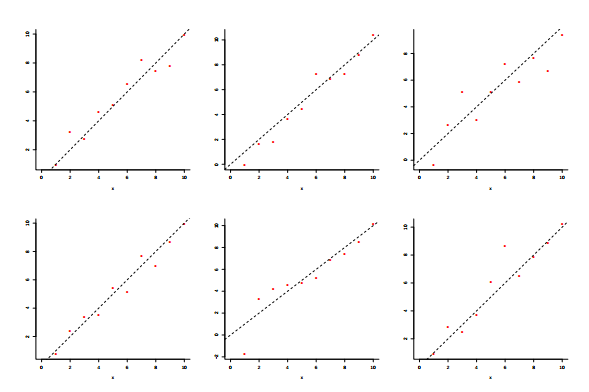
\includegraphics[scale=0.6]{img/6ejemplosRegresion.png}
\end{center}

Vemos que obviamente las rectas no son las mismas. Esto se debe al $ε_i$ introducido. ¿Cuáles son los valores que toman $β_1$ y $β_0$? Habiendo repetido el experimento 1000 veces, obtenemos los siguientes histogramas:

\begin{center}
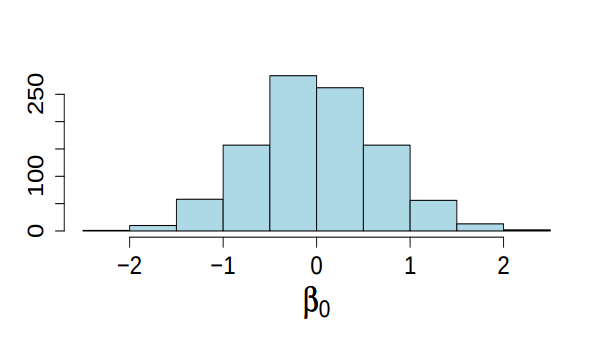
\includegraphics[scale=0.3]{img/1000vecesb0.png}
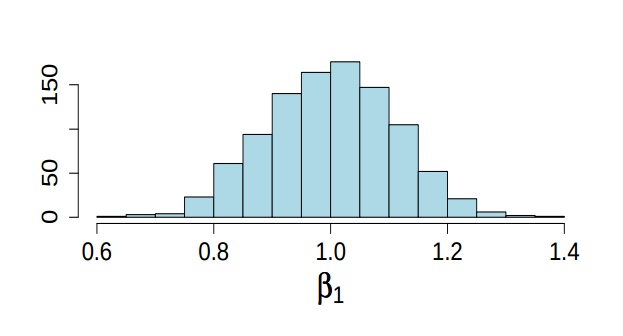
\includegraphics[scale=0.3]{img/1000vecesb1.png}
\end{center}

Vemos que no siempre es el mismo valor. Sabemos (por cómo hemos construido los datos) que $β_0 = 0$ y $β_1 = 1$, pero nuestra manera de calcularos (debido a $ε_i$) no siempre nos da el valor concreto.


\end{example}

El ejemplo anterior nos muestra que en realidad, estamos estimando $β_i$, aunque no nos guste y ahora tenemos que plantearnos ¿Cómo de buenos son nuestros estimadores? Tal vez son una mierda, o tal vez son insesgados.

Para ello, vemos que al haber añadido un error $\epsilon_i \sim N(0,σ^2)$, tenemos:

\[
Y_i = β_0 + β_1x + ε_i \implies Y_i \equiv N(β_0 + β_1X_i, σ^2)
\]


\subsubsection{Estimando $β_1$}

\begin{prop}
Nuestro estimador ``pendiente de la recta de mínimos cuadrados:'' $\hat{β_1}$  cumple

\[
\hat{β_1} \equiv N\left(β_1,\frac{σ^2}{S_{xx}} \right)
\]

\end{prop}

\begin{proof}
Él en clase lo ha hecho al revés. Muchos cálculos para llegar a la conclusión, pero aquí molamos más. En algún momento \textcolor{red}{revisará} alguien los apuntes y completará.

\begin{itemize}
	\item $\esp{\hat{β_1}} = β_1$
	\item $\var{\hat{β_1}} = ... = \displaystyle\frac{σ^2}{S_{xx}}$
\end{itemize}
\end{proof}

\subsubsection{Estimando $β_0$}

\begin{prop}
Nuestro estimador ``término independiente de la recta de mínimos cuadrados:'' $\hat{β_0}$  cumple

\[
\hat{β_0} = N\left(β_0 , σ^2 \left( \frac{1}{n} + \frac{\gor{x}^2}{S_{xx}}\right)  \right)
\]
\end{prop}

\begin{proof}
\begin{itemize}
	\item $\esp{\hat{β_0}} = β_0$
	\item
	$\var{\hat{β_0}} = \var{\gor{Y}} + \var{\hat{β_1}\gor{X}} - 2 \cov{\gor{Y},\hat{β_1}\gor{X}}$

 	\subitem Calculamos: $\cov{\gor{Y},\hat{β_1}\gor{X}}$ utilizando cosas del tema 1

 	\[
		\cov{\gor{Y},\hat{β_1}\gor{X}} = \cov{\frac{1'_n \gor{Y}}{n},α\gor{Y}} = \frac{1}{n}1'_nσ^2
 	\]
 	debido a que $α = 0$.

 	Ademas de ser incorrelados, son \textbf{independientes}. ¿Porqué? Porque conjuntamente son normales, es decir \[
 		\begin{pmatrix} \gor{Y} \\ \hat{β_1} \end{pmatrix} \equiv A\gor{Y} \equiv N_2
 	\]
\end{itemize}

\end{proof}


\textbf{Conclusiones:}
\begin{align*}
\gor{Y} &\text{ es independiente de } \hat{β_1}\\
\hat{β_1} &\equiv \left(β_1,\frac{σ^2}{S_{xx}}\right)\\
\hat{β_0} &\equiv \left(β_0,σ^2 \left( \frac{1}{n} + \frac{\gor{x}^2}{S_{xx}}\right)\right)
\end{align*}

¿Son estas las variables $\hat{β_1} $ y $\hat{β_0}$ normales una normal conjunta? Sí, \textbf{sí son una normal conjunta}. Una manera que tenemos de saber si es una normal conjunta es si son independientes, y en este caso no lo son.  Intuitivamente es fácil de ver. En una recta, si aumentamos la pendiente (y estamos en el primer cuadrante) entonces el término independiente disminuye.

Esta dependencia tiene que aparecer. Vamos a estudiar la covarianza entre los estimadores:

\[
\cov{β_1,β_0} = \cov{\gor{Y} - \hat{β_1}\gor{x}, \hat{β_0}} = ... = -\gor{x}\frac{σ^2}{S_{xx}}
\]


Pero sabemos que sí son una normal bidimensional porque toda combinación lineal de nuestros parámetros de la recta es una variable aleatoria (la variable regresora $\hat{Y}$) normal.


\subsubsection{IC y Contrastes para $β_1$}
\label{subsubsec:ICparaB1}

Recordamos que \[ \hat{β}_1 \equiv N\left(β_1,\frac{σ^2}{S_{xx}}\right)\]

Podemos normalizar y buscar una cantidad pivotal (como hacíamos en estadística I)

\[
\frac{\hat{β_1} - β_1}{\frac{σ}{\sqrt{S_{xx}}}} \equiv N\left(0,1\right)
\]

Pero aquí nos encontramos con que necesitamos $σ$, la varianza de los errores. Esta varianza a menudo no es conocida (porque no sabemos con exactitud cuál es la recta verdadera) y tenemos que estimarla.

Para estimarla, parece razonable usar \[ \hat{σ} = S_R =\frac{\sum_{i=1}^n e_i^2}{n-2}\]

\begin{expla}
Recordamos que para que estimar la varianza, utilizamos (por el lema de Fisher) $n-1$ de denominador para que el estimador sea insesgado. Esto sale de que en la demostración, hay una matriz de rango $n-1$ ya que existe una restricción.

Siguiendo este razonamiento, en este caso tenemos 2 restricciones\footnote{$\sum e_i = 0$ y $\sum e_ix_i = 0$}, por lo que si lo demostráramos rigurosamente, aparecería una matriz de rango $n-2$ y por eso es el denominador. De esta manera, conseguimos un estimador insesgado.

\end{expla}

Además, $S_R$ se denomina \concept{Varianza\IS residual}

\begin{prop}
Una pequeña generalización del lema de Fisher:
\[
\frac{(n-2)S_{R}^2}{σ^2} \equiv \chi_{n-2}^2
\]

Además, es independiente de $\hat{β_1}$

\end{prop}



\begin{proof}
Esta proposición es un caso particular de un teorema que veremos más adelante.
\end{proof}


Llamamos
\[ P_{R} = \frac{\hat{β_1}-β_1}{\frac{S_R}{\sqrt{S_{xx}}}}\]
\[ P_σ = \frac{\hat{β_1}-β_1}{\frac{σ}{\sqrt{S_{xx}}}}\]

Sabemos que $P_σ \sim N(0,1)$. Pero, al estimar ¿Se mantiene$P_R \sim N(0,1)$?

Al estimar $σ$,  $P_{R}$ no tiene porqué ser exactamente $N(0,1)$. Si $n\to ∞$, entonces $S_R = σ$ y entonces $P_σ = P_R = N(0,1)$, pero para otros valores de $n≠∞$...

Por ello, nos vemos en la necesidad de manipular $P_R$ algebraicamente a ver si conocemos qué distribución tiene (que debería ser algo cercano a una normal, ya que estamos estimando $σ$ con un estimador insesgado. Tal vez las colas de la distribución son menos pesadas y podríamos esperar que fuera una $t$)

\label{Cuentas:largas}

\[
\displaystyle\frac{\hat{β_1}-β_1}{\displaystyle\frac{S_R}{\sqrt{S_{xx}}}} = \displaystyle\frac{\hat{β_1}-β_1}{\displaystyle\frac{σ}{\sqrt{S_{xx}}}\frac{S_R}{σ}} = \left( \displaystyle\frac{\hat{β_1}-β_1}{\displaystyle\frac{σ}{\sqrt{S_{xx}}}} \right)\displaystyle\frac{1}{\displaystyle\frac{S_R}{σ}} = \displaystyle\frac{ \displaystyle\frac{\hat{β_1}-β_1}{\frac{σ}{\sqrt{S_{xx}}}} }{\displaystyle\frac{S_R}{σ}}
\]

En el numerador tenemos una $N(0,1)$ y en el denominador la raíz de una $\chi^2$ dividida por sus grados de libertad (por la proposición anterior). Esto es por definición una $t$ (T-Student) con los mismos grados de libertad que la $\chi^2$, es decir $n-2$. (\href{https://en.wikipedia.org/wiki/Student%27s\_t-distribution#Characterization}{Wikipedia})


\begin{prop}
Podemos calcular el intervalo de confianza  para la pendiente de la recta, utilizando la fórmula de intervalo de confianza

\[
IC_{1-α}(β_1) \equiv \left[ \hat{β_1} \mp t_{n-2,\frac{α}{2}}\frac{S_R}{\sqrt{S_{xx}}}\right] = \left[ \hat{β_1} \mp \mathcal{Z}\frac{σ}{\sqrt{S_{xx}}}\right] %\equiv \left[ \gor{Y} \mp \t_{n-1,\frac{α}{2}}\frac{S_R}{\sqrt{n}} \right]
\]
\end{prop}

\subsubsection{Contraste en R}

\label{example:R-output}
\begin{lstlisting}[style=mystyle]
# Ajusta el modelo
regresion = lm(Fracaso~Renta)
summary(regresion)

lm(formula = Fracaso ~ Renta)

Residuals:	Min		1Q			Median		3Q		Max
				-7.8717 -3.7421		0.5878	3.0368	11.5423
---
Coefficients:	Estimate Std.	Error 	t-value		Pr(>|t|)
(Intercept)		38.4944				3.6445	10.562		8.37e-10 ***
Renta 				-1.3467				0.2659	-5.065		5.14e-05 ***
---
Signif. codes: [...]
Residual standard error: 4.757 on 21 degrees of freedom
Multiple R-Squared: 0.5499,
Adjusted R-squared: 0.528
\end{lstlisting}


Aquí, la fila de \textit{intercept} es el término independiente y renta es la pendiente. Además, los p-valores son para el contraste $\hat{β_i} = 0$, dentro de la hipótesis $β_i \geq 0$. \footnote{Si queremos contrastar si es positivo, nos vamos al caso límite que lo separa y contrastamos eso}.

En este caso, el p-valor para $H_0: \hat{β_1}=$ es $5.14e-5$, con lo que no podemos rechazar la hipótesis.


\subsubsection{Predicciones}

Sea $(x_1,y_1),...,(x_n,y_n) \to y_i = β_0 + β_1x_i + ε_i$.

Dado una nueva observación $x_0$, tenemos 2 problemas para predecir:

\begin{itemize}
	\item \textbf{Inferencia sobre $m_0 \equiv \esp{y_0 | x_0} = β_0 + β_1x_0$}

	En este caso, $$\hat{m_0} = \hat{β_0} + \hat{β_1}x_0$$

	¿Cómo es este estimador?

	\[\esp{\hat{m_0}} = β_0 + β_1x_0 = m_0\]
	\[\var{\hat{m_0}} = ... = σ^2\left[\frac{1}{n} + \frac{(x_0-\bar{x})^2}{S_{xx}} \right] \]

	\subitem Intuitivamente, lo que significa el segundo sumando de la varianza es que ``cuanto más cerca esté $x_0$ de la media, mejor será la estimación''.

	\textbf{Conclusión:}

	\[
		\hat{m_0} \sim N\left( m_0, σ^2\left[\frac{1}{n} + \frac{(x_0-\bar{x})^2}{S_{xx}} \right]\right)
	\]



	\subitem \textbf{Intervalo de confianza} para $m_0$ utilizando la fórmula de intervalos de confianza:

	\[
IC_{1-α}(m_0) \equiv \left[ \hat{m_0} \pm t_{n-2,\frac{α}{2}}S_R\sqrt{\frac{1}{n} + \frac{(x - \gor{x})^2}{S_{xx}}}\right]
\]

	\item \textbf{Predecir $Y_0$} usamos de nuevo:

	\[
\hat{Y_0} = \hat{β_0} + \hat{β_1}x \to Y_0 - Y \equiv N\left( 0, σ^2\left( 1 + \frac{1}{n}+  \frac{(x-\gor{x})^2}{S_{xx}}\right) \right)
	\]

	Donde la varianza ha sido calculada:

	\[
	\var{Y_0 - \hat{Y_0}} = \underbrace{\var{Y_0}}_{σ^2} - \var{\hat{Y_0}} + \underbrace{2 \cov{Y_0,\hat{Y_0}}}_{ = 0 \text{ (indep.) }} = σ^2 + σ^2\left( \frac{1}{n}+  \frac{(x-\gor{x})^2}{S_{xx}} \right)
	\]


	Este es un problema más complicado, ya que tenemos que tener en cuenta el término de error $ε_i$ y es por esto que aparece el 1 en la varianza. Tenemos que tener en cuenta la incertidumbre.

	Estandarizando y cambiando $σ$ por $S$, tenemos:

	\[
	\frac{Y_0 - \hat{Y_0}}{S_r \sqrt{1 + \frac{1}{n} + \frac{(x-\gor{x})^2}{S_{xx}}}} \equiv t_{n-2}
	\]

	Ya que tenemos una normal estandarizada dividida por su .... que por definición, es una $t$ de student.

	Ahora, vamos a construir el \concept{intervalo de predicción} (cambia ligeramente la interpretación)

	\[
1 - α = P\left\{ -t_{n-2;\frac{α}{2}} < \frac{Y_0 - \hat{Y_0}}{...} < t_{n-2;\frac{α}{2}}    \right\} = P \left\{ Y_0 \in \left[ \hat{Y_0} \pm t_{n-2;\frac{α}{2}} S_R \sqrt{1+\frac{1}{n}+...} \right]  \right\}
	\]
\end{itemize}

Ahora vamos a hacer unos ejemplos numéricos.

\begin{example}Seguimos con el ejemplo de la renta.
\begin{problem}
\begin{center}
\begin{tabular}{c|c|c}
&media&desviación típica\\\hline
\% fracaso & 20.73 & 6.927\\
renta &13.19  & 3.814
\end{tabular}
La renta está expresada en miles de euros.
\end{center}


\ppart IC para $β_1$ de nivel $95\%$.
\ppart IC para \% de fracaso medio si la renta es de $14.000$ euros.


Es parte del enunciado la salida de ``R'' incluida en: \ref{example:R-output}

\solution
\spart

\[
IC_{1-α}(β_1) = \left[-1.3467 \mp t_{21;0.025} · (0.2659)\right]
\]

Donde el $-1.3467$ es el estimador $\gor{β_1}$ que obtenemos de la salida de $R$. Lo mismo el $0.2659$, que es el error típico.

\spart
\[ \gor{Y_0} = 38.49 - (1.3467) · \underbrace{14}_{x_0} = 19.64\]

Siendo este el estimador, vamos a construir el intervalo de confianza. \footnote{Podría ser que nos pidieran el intervalo de predicción, pero en ese caso estarían pidiendo el intervalo de ...... para predecir. Además, nos están dando un $x_0$ que para predicción no lo tenemos}

\[
IC_{1-α}(m_0) = \left[19.64 \mp (2.06)(4.757)\sqrt{\frac{1}{23}+\frac{(14-13.19)^2}{S_{xx}}}\right]
\]
Donde $S_{xx} = 320.06$ y podemos calcularlo despejando de:

\[
E.T.(\gor{β_1}) = \sqrt{\frac{S_R^2}{S_{xx}}} \to \sqrt{S_{xx}} = \frac{4.757}{0.2659} \to S_{xx} = 320.06
\]
Donde $E.T.(\gor{β_1})$ es el error típico dado por \textit{R}. En este caso es $0.2659$y $S_R^2 = 4.757^2$

También podríamos utililzar $S_x = \frac{S_{xx}}{n-1}$, sabiendo que $S_x^2 = \frac{n}{n-1}σ^2$. Sabemos que $S_x = 3.814$ por ser la renta la variable explicativa, es decir, las $x$ de nuestro modelo de regresión.

\[
\frac{n}{n-1}\left(3.814\right)^2 = \frac{S_{xx}}{n-1} \to S_{xx} = 21·\left(3.814^2·\frac{22}{21}\right) = 320.03
\]
\end{problem}


\end{example}


\obs Todos estos cálculos y todas estas fórmulas se basan en muchas hipótesis (como que la distribución del error sigue una distribución normal). Pero podría ser que esto no ocurriera y estuviéramos suponiendo un modelo falso. Para ello, en estadística existe el \concept{Diagnóstico del modelo}. Este diagnóstico, consiste en comprobar si las hipótesis del modelo son \textbf{aceptables} para los datos disponibles. ¡Ojo! Aceptable... Puede haber muchos modelos aceptables para un mismo conjunto de datos.

Este diagnóstico se suele basar en el análisis de los residuos del modelo.

\begin{example}
	Vamos a ver a ojo unos cuantos ejemplos. Vamos a utilizar que $\corr{e,\gor{y}} = 0$ bajo el modelo (como calculamos anteriormente)

\begin{center}
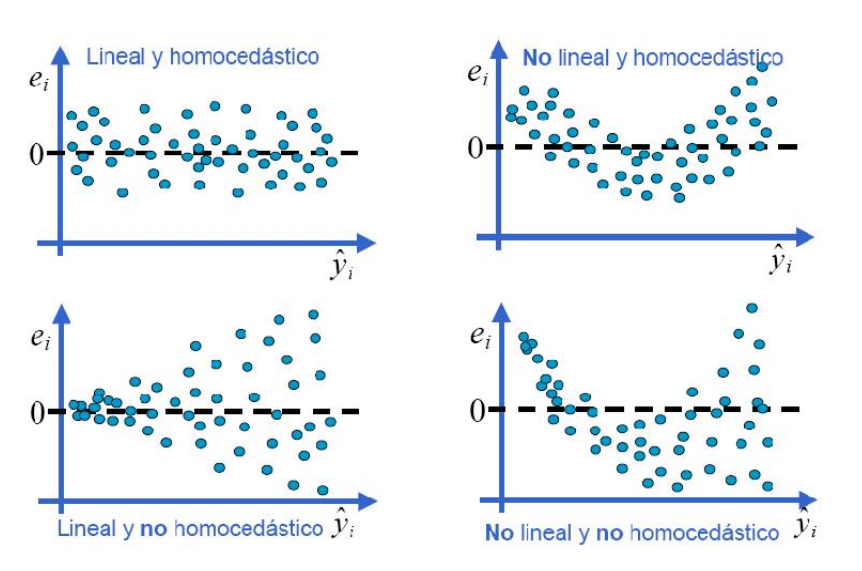
\includegraphics[scale=0.5]{img/diagmodelo.png}
\end{center}

De estos 4 gráficos, el bueno es el primero, ya que los demás no cumplen alguno.
\end{example}

\begin{example}
Vamos a ver otro ejemplo, donde arriba están los datos y abajo los residuos. Mirando sólo la fila de arriba podríamos saber si nuestro modelo para la regresión se cumple o sino.


\begin{center}
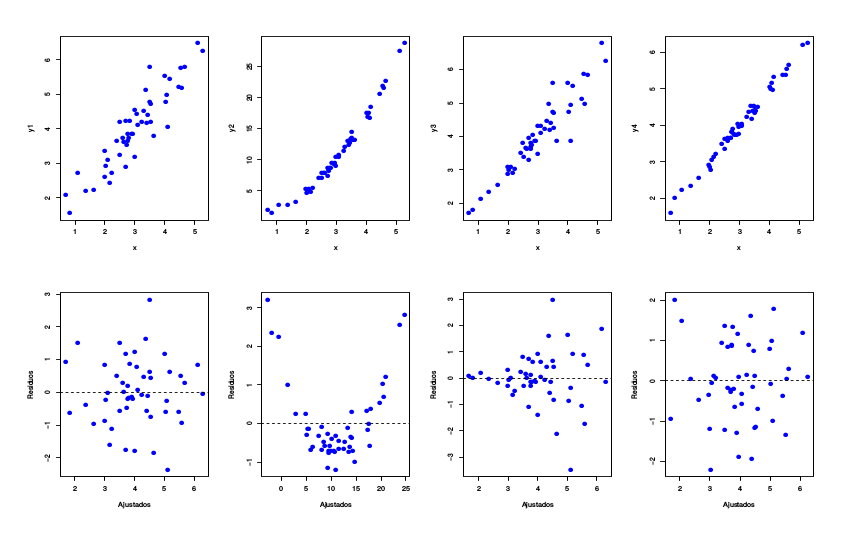
\includegraphics[scale=0.5]{img/diagmodelo_2.png}
\end{center}

Vemos que el primero y el último si tienen este modelo como aceptable, ya que en los residuos no hay ningún patrón (y se cumple que la correlación es 0).

En el segundo, podríamos suponer que es bueno, pero al diagnosticar el modelo mirando los residuos, vemos que no. El diagnóstico del modelo \textbf{magnifica los errores}.

En el cuarto, vemos más claro que es heterocedástico y que no se cumple el modelo supuesto.
\end{example}

En regresión múltiple veremos que no podemos ver los datos, ya que son demasiadas variables, pero sí podemos estudiar los residuos como acabamos de hacer en los ejemplos anteriores.


\subsection{Regresión lineal múltiple}

El ejemplo que vamos a estudiar en regresión múltiple es el consumo de gasolina en EEUU intentando predecirlo a partir de unas cuantas variables. Las variables regresoras son:

\begin{center}
\begin{tabular}{cccccccc}
State&Drivers&FuelC&Income&Miles&MPC&Pop&Tax\\\hline
AL&3559897&2382507&23471&94440&12737.00&3451586&18.0\\
AK&472211&235400&30064&13628&7639.16&457728&8.0\\
AZ&3550367&2428430&25578&55245&9411.55&3907526&18.0
\end{tabular}
\end{center}


Estos son los datos que obtenemos de $R$:

\begin{lstlisting}[style=mystyle]
reg <- lm(FuelC ~ Drivers+Income+Miles+MPC+Tax, data=fuel2001)
summary(reg)
Call:
lm(formula = FuelC ~ Drivers + Income + Miles + MPC + Tax, data = fuel2001)
Coefficients:
Estimate	Std.Error	t	value	Pr(>|t|)
(Intercept)	-4.844e+05	8.102e+05	-0.598	0.552903
Drivers	6.144e-01	2.229e-02	27.560	<	2e-16
Income	7.526e+00	1.611e+01	0.467	0.642587
Miles	5.813e+00	1.587e+00	3.664	0.000652
MPC	4.643e+01	3.488e+01	1.331	0.189820
Tax	-2.114e+04	1.298e+04	-1.629	0.110298
---
Residual standard error: 394100 on 45 degrees of freedom
Multiple R-squared: 0.9808, Adjusted R-squared: 0.9787
F-statistic: 459.5 on 5 and 45 DF, p-value: < 2.2e-16
\end{lstlisting}

\subsubsection{Notación}


\begin{itemize}
	\item $n$ es el número de observaciones, en este caso, el número de estados.
	\item $k$ es el número de atributos.
	\item $ε_i \sim N(0,σ^2)$
	\item $n\geq k+2$: esta hípótesis  es muy necesaria.\footnote{En la estadística, habría que rehacer el modelo para cuando $k>n$. ¿Y cuándo $k>n$? ¿Cuándo puede ocurrir esto? Cada vez más hay más información para cada individuo. En estudios genéticos por ejemplo, que hay millones de genes pero no se pueden hacer el estudio con millones de personas... \textbf{LA MALDICIÓN DE LA DIMENSIONALIDAD} que decimos en Introducción previa a los Fundamentos Básicos del Aprendizaje Automático.\\ Una posible solución al problema es un algoritmo que filtre los atributos que son importantes.}
\end{itemize}

Regresión simple es un caso particular de múltiple, tomando $k=1$.

\subsubsection{Modelo}

Tenemos una muestra de $n$ observaciones de las variables $Y$ y $X_1,…,X_k$. Para la observación $i$, tenemos el vector $(Y_i,x_{i1},x_{i2},…,x_{ik})$.

El modelo de regresión lineal múltiple supone que:
\[Y_i=β_0+β_1x_{i1}+…+β_kx_{ik}+ε_i,\ i=1,...,n\]

donde las variables de error $ε_i$ verifican:
\begin{enumerate}
\item $ε_i$ tiene media cero, para todo $i$.
\item Var($ε_i$) = $σ^2$, para todo $i$ (homocedasticidad).
\item Son variables independientes.
\item Tienen distribución normal.
\item $n ≥ k + 2$ (hay más observaciones que parámetros).
\item Las variables $X_i$ son linealmente independientes entre sí (no hay colinealidad).
\end{enumerate}

Las 4 primeras hipótesis se pueden reexpresar así: las observaciones de la muestra son independientes entre sí con
\[Y_i \equiv N(β_0 +β_1x_{i1} +...+β_kx_{ik},σ),\ i=1,...,n\]

En forma matricial:

\[
	\begin{pmatrix}
		Y_1\\
		Y_2\\
		\vdots \\
		Y_n
	\end{pmatrix}
	=
	\begin{pmatrix}
		1 & x_{11} & … & x_{1k} \\
		1 & x_{21} & … & x_{2k} \\
		\vdots & \vdots &  & \vdots \\
		1 & x_{n1} & … & x_{nk}
	\end{pmatrix}
	\begin{pmatrix}
		β_1\\
		β_2\\
		\vdots \\
		β_n
	\end{pmatrix}
	+
	\begin{pmatrix}
		ε_1\\
		ε_2\\
		\vdots \\
		ε_n
	\end{pmatrix}
\]


De forma más compacta, el modelo equivale a:
\[Y =Xβ+ε,\ ε \equiv N_n(0,σ^2I_n) \iff Y \equiv N_n(Xβ,σ^2I_n)\]

\begin{defn}[Matriz de diseño]
	La matriz $X$ se conoce como matriz de diseño
\end{defn}

\subsubsection{Estimación de los parámetros del modelo}

La pregunta que lógicamente se nos viene a la cabeza en este momento es: ¿Cómo estimar $β$ a partir de $Y$ y $X$?. Para ello nos serviremos de la interpretación geométrica del modelo:

Sea $\mathcal{V} ⊂ R^n$ el subespacio vectorial generado por las columnas de la matriz de diseño $X$ ($\dim(\mathcal{V}) = k + 1$).
\[μ∈\mathcal{V} \iff ∃β∈R^{k+1} : μ=Xβ\]
El modelo equivale a suponer $Y \equiv N_n(μ, σ^2I_n)$, donde $μ ∈ \mathcal{V}$.

\newpage
\begin{figure}[hbtp]
	\centering
	\inputtikz{proyecta_V}
\end{figure}

Con esto, parece razonable estimar $µ$ mediante la proyección ortogonal de $Y$ sobre $\mathcal{V}$ para obtener $\hat{Y} = X\hat{β}$. Equivalentemente: $\norm{Y-X\hat{β}}^2 \leq \norm{Y-Xβ}^2, ∀β\in ℝ^{k+1}$

\begin{defn}[Estimador mínimos cuadrados]

	Al $\hat{β}$ que minimiza
	\[\norm{Y - Xβ}^2 = \sum_{i=1}^n (Y_i - β_0 - β_1x_{i1} - … - β_kx_{ik})^2\]
	se le denomina estimador de mínimos cuadrados.
\end{defn}

Veamos qué podemos sacar de lo visto hasta ahora para averiguar quién es exactamente $\hat{β}$:

Para que $\hat{Y}$ sea la proyección de $Y$ sobre $\mathcal{V}$ es necesario y suficiente que se satisfagan las ecuaciones normales:

\begin{defn}[Ecuaciones normales]
	Tomando $e = Y - \hat{Y}$ como el vector residuo, las ecuaciones normales se satisfacen si:
	\[X'(Y - \hat{Y})=0 \iff X'e = 0\]
\end{defn}

Que se satisfagan estas ecuaciones es equivalente a decir que la resta $Y - \hat{Y}$ da un vector perpendicular a la base $\mathcal{V}$. Sustituyendo $\hat{Y} = X\hat{β}$:

\[X'(Y - X\hat{β}) = 0 \iff X'Y = X'X\hat{β}\]

Ya que las filas de $X'$ (las columnas de $X$) son independientes, sabemos que $X'X$ tiene rango completo y por tanto es invertible. Y llegamos a la expresión para nuestro estimador de mínimos cuadrados $\hat{β}$:
\begin{equation}
	\boxed{\hat{β} = (X'X)^{-1}X'Y}
\end{equation}


\begin{obs}
	En regresión simple se tiene que:
	\[
		X\equiv
		\begin{pmatrix}
			1 & x_1\\
			\vdots & \vdots \\
			1 & x_n
		\end{pmatrix}
		\text{ y que: }
		X'X =
		\begin{pmatrix}
			n & \sum x_i \\
			\sum x_i & \sum x_i^2
		\end{pmatrix}
	\]
\end{obs}

Con lo visto hasta el momento sabemos que $\hat{Y} = X\hat{β} = X(X'X)^{-1}X'Y$, es decir, que nuestra $\hat{Y}$ está expresada como producto de $Y$ por una matriz que llamaremos:

\begin{defn}[Hat matrix]
	\[H = X(X'X)^{-1}X'\]
	se conoce como hat matrix, puesto que da $Y$ gorro: $\hat{Y} = HY$.
\end{defn}

La hat matrix $H$ tiene las siguientes \textbf{propiedades}:
\begin{itemize}
	\item Es matriz de proyección ortogonal sobre $\mathcal{V}$.
	\item Es simétrica e idempotente.
	\item Tiene rango $k+1$ (la dimensión del espacio $\mathcal{V}$ sobre el que proyecta).
\end{itemize}

\begin{obs}
	Podemos servirnos de la hat matrix para expresar el vector de residuos:
	\[e = Y - \hat{Y} = Y - HY = (I - H)Y\]
	Donde $(I-H)$ es una matriz simétrica e idempotente con rango $rg(I-H)=~n-~(k~+~1)$, que proyecta sobre el espacio ortogonal $\mathcal{V}^\perp$.
\end{obs}

Para acabar esta sección enumeramos algunas propiedades de los parámetros:
\begin{itemize}
\item $\hat{β}$ es el estimador de máxima verosimilitud (EMV) de $β$:
\[L(β,σ)= \left(\frac{1}{\sqrt{2π}σ}\right)^n exp\left\{-\frac{1}{2σ^2} \norm{Y−Xβ}^2 \right\}.\]

\item El EMV de $σ^2$ es:
\[\hat{σ}^2 = \frac{\norm{Y−Xβ}^2}{n} = \frac{\norm{e}^2}{n} = \frac{\sum_{i=1}^n e_i^2}{n}\]

\item El vector $\hat{β}$ tiene distribución $N_{k+1}(β, σ^2(X′X)^{−1})$ (en la siguiente sección se demuestra).
\end{itemize}

\subsubsection{Estudio de la varianza residual}
Un estimador insesgado de $σ^2$ es la varianza residual $S_R^2$ , es decir, la suma de los residuos al cuadrado, corregida por los grados de libertad apropiados (en este caso $n-\dim{(\mathcal{V})}$):
\[S_R^2 = \frac{\sum e_i^2}{n-(k+1)} = \frac{\norm{e}^2}{n-k-1} = \frac{\norm{Y - \hat{Y}}^2}{n-k-1}\]

Si nos fijamos en que:
\[\norm{Y - \hat{Y}}^2 = Y'(I-H)(I-H)Y = Y'(I-H)Y\]

y sabiendo que la matriz $I-H$ es simétrica e idempotente, si recordamos la proposición \ref{prop:tema1_pepino} y demostramos $μ(I-H)μ'=0$, podemos determinar que la distribución de $S_R^2$:

Dado que $μ∈\mathcal{V}$ y sabiendo que $μ=XB$:
\[(I-H)μ = (I-H)XB = 0\]
Ya que el vector $(I-H)$ proyecta sobre $\mathcal{V}^\perp$.

Así llegamos a que:
\[\frac{\norm{Y-\hat{Y}}^2}{σ^2} = \frac{Y'(I-H)Y}{σ^2}=\]
\begin{equation}
	\boxed{\frac{(n-k-1)S_R^2}{σ^2} \equiv χ_{n-k-1}^2}
\end{equation}


Además si tomamos esperanzas en ambos lados de la igualdad obtenemos:
\[\frac{(n-k-1)·\mathbb{E}(S_R^2)}{σ^2} = n-k-1\]
\begin{equation}
	\boxed{\mathbb{E}(S_R^2) = σ^2}
\end{equation}

Lo siguiente que haremos es mirar si $\hat{β}$ y $S_R^2$ \textbf{son independientes}. Esto es cierto dado que se cumple que $(X'X)^{-1}X' · (I-H)=0$:
\[(X'X)^{-1}X' · (I-H) = (X'X)^{-1}X' - (X'X)^{-1}X' · X(X'X)^{-1}X' =0\]

\begin{obs}
	El lema de Fisher \ref{lemma:fisher} no es más que el resultado de aplicar los resultados vistos en esta sección al caso particular del modelo:
	\[y_i = β_0 + ε_i \iff X=\begin{pmatrix}1\\ \vdots \\ 1\end{pmatrix}\]
	En este caso tenemos que $\dim{(V)}=1$
\end{obs}


\subsubsection{Distribución de $\hat{β}$ y contrastes de hipótesis individuales sobre los coeficientes $\hat{β}_i$}
\[\esp{\hat{β}} = (X'X)^{-1}X' \underbrace{Xβ}_{\esp{Y}} = β\]
\[\var{\hat{β}} = σ^2I_n · (X'X)^{-1}X' · X(X'X)^{-1} = σ^2(X'X)^{-1}\]

Como $\hat{β}$ es una combinación lineal de $Y$ (que sigue una distribución normal):

\[
\hat{β} \equiv N_{k+1}\left(β,σ^2(X'X)^{-1}\right)
\]

Y la regresión simple, es un caso particular de esta fórmula.

\textbf{Notação}: $q_{ij}\equiv$ entrada $i,j$ de la matriz $(X'X)^{-1}$

\paragraph{Consecuencias:}

\begin{itemize}
	\item ¿Cuál es la distribución marginal de $\hat{β_j}$ a partir de la que hemos visto de la conjunta? Como vimos en el tema 1, es también una normal, con el correspondiente valor del vector $β$ como media y el elemento $j,j$ de la diagonal.
	\[ \hat{β}_j \equiv N\left(β_j, σ^2q_{jj}\right)\]

	Ahora, podemos estandarizar:

	\[
	\frac{\hat{β_j}-β_j}{σ\sqrt{q_{jj}}} \equiv N(0,1)
	\]

	Y utilizando que $S_R$ es independiente de $σ$ y la definición de $t-$student tenemos:

	\[
	\frac{\hat{β_j}-β_j}{S_R\sqrt{q_{jj}}} \equiv t_{n-k-1}
	\]

	¿Cuál es el intervalo de confianza?

	\[
		IC_{1-α}(β_j) \equiv \left[\hat{β_j}\mp t_{n-k-1;\frac{α}{2}}\underbrace{S_R\sqrt{q_{jj}}}_{\text{Error típico de }β_j} \right]
	\]

	Y, como en regresión simple, estudiamos $H_0 : β_j = 0$:
	\[
		R = \left\{ \frac{\abs{\hat{β}_j}}{S_R\sqrt{q_{jj}}} > t_{n-k-1;\frac{α}{2}} \right\}
	\]
\end{itemize}

En las traspas encontramos una salida de regresión múltiple de $R$. La columna \textit{estimate} es el vector $\hat{β}$, el p-valor es del contraste $H_0 : β_j = 0$.


\subsubsection{Combinaciones lineales de los coeficientes} Vamos a querer constrastar cosas del estilo ¿las 2 variables influyen igual?

Para ello, transformamos eso en $H_0: β_1 = β_2 \to H_0 : β_1 - β_2 = 0$, entonces tenemos una combinación lineal $a∈ℝ^{k+1}$, tal que $H_0:a'\hat{β} = 0$

Para poder hacer esto, lo primero ha sido estimar $\hat{β}$ y lo siguiente será saber su distribución.

\[a'\hat{β} = N\left(a'β,\underbrace{σ^2a'(X'X)^{-1}a}_{\left(E.T.(a'\hat{β})\right)^2}\right) \to \frac{a'\hat{β} - a'β}{S_R\sqrt{a'(X'X)^{-1}a}} \equiv t_{n-k-1}\]

Y con esto, ya podemos construir el intervalo de confianza para una combinación lineal de los parámetros:

\[
IC_{1-α}(a'β) = \left[ a'\hat{β} \mp t_{n-k-1;\frac{α}{2}}E.T.(a'\hat{β}) \right]
\]

La región de rechazo correspondiente es:

\[
R = \left\{ \frac{a'\hat{β}}{S_R\sqrt{σ^2a'(X'X)^{-1}a}} >  t_{n-k-1;\frac{α}{2}} \right\} = \left\{ \frac{a'\hat{β}}{E.T.(\hat{β})} >  t_{n-k-1;\frac{α}{2}} \right\}
\]

\paragraph{Ejercicio:} ¿Y si queremos hacer un contraste unilateral $a'β > 0$?

\subsubsection{Inferencia sobre subconjuntos de coeficientes}

Todos los contrastes hechos hasta ahora son muy fáciles porque se basan en una única normal. Nuestros contrastes han sido del tipo $β_i = 0$. En esta sección vamos a estudiar contrastes del tipo $H_0: β_1 = 0, β_3 = 0$.

La primera aproximación puede ser calcular la región de confianza de $β_1$ y la de $β_3$ y tomar la intersección. Es decir:

\begin{center}
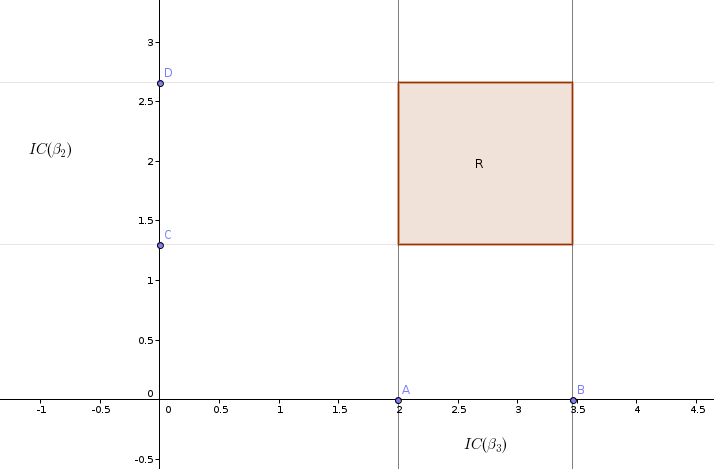
\includegraphics[scale=0.5]{img/confianzamultivariantemal.png}
\end{center}

 Pero al no ser independientes, no estamos teniendo en cuanto las correlaciones, la información que me da saber $β_1$ para saber $β_3$.

\begin{center}
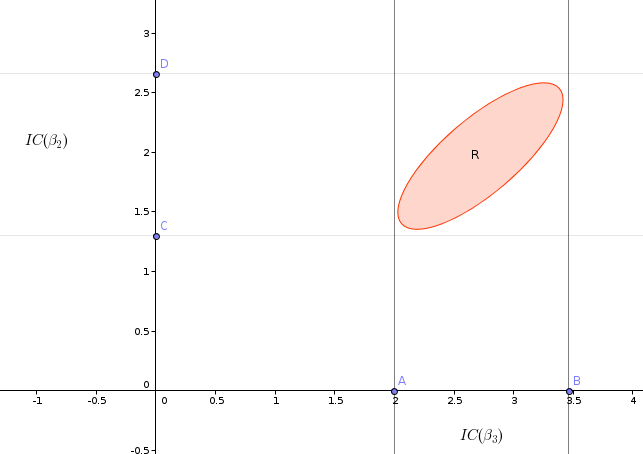
\includegraphics[scale=0.5]{img/confianzamultivariantebien.png}
\end{center}

\paragraph{Vamos a ello formalmente:}
\newcommand{\bpp}{β_{(p)}}
\newcommand{\hbpp}{\hat{β}_{(p)}}
\newcommand{\fpnk}{F_{p,n-k-1}}
Sea $β_{(p)}$ un conjunto de coeficientes de $β$. Sea $\hbpp$ el correspondiente subconjunto de estimadores.

Sea $Q_q$ la submatriz de $(X'X)^{-1}$ cuyas filas y columnas corresponden a las coordenadas del vector $\bpp$.

\[\hbpp \equiv N_p \left( \bpp, σ^2Q_p \right)\]

Si este es nuestro estimador, vamos a estandarizarlo (utilizando propiedades del tema 1).

\[
\frac{(\hbpp - \bpp)'Q_p^{-1}(\hbpp - \bpp)}{σ^2}\equiv \chi^2_p
\]

Tenemos el problema de que no conocemos $σ$ y tenemos que estimarlo. Para ello, vamos a seguir un proceso parecido a \ref{Cuentas:largas}. Para ello necesitamos:

\begin{defn}[Distribución $F_{n,m}$]

\[
F_{n,m} \equiv \frac{\chi^2_m / m}{\chi^2_n / n}
\]

Es muy habitual que aparezca la $F$ al comparar varianzas.
\end{defn}

Sabiendo lo que es una $F$, vamos a estudiar qué ocurre al cambiar $σ$ por $S_R$

\[
\frac{(\hbpp - \bpp)'Q_p^{-1}(\hbpp - \bpp)}{S_R^2} = \frac{\frac{(\hbpp - \bpp)'Q_p^{-1}(\hbpp - \bpp)}{σ^2}}{\frac{S_R^2}{σ^2}}
\]

En el numerador tenemos una $\chi^2_p$, pero nos faltaría dividir por los grados de libertad para tener una $F$, entonces:

\[
\frac{\frac{(\hbpp - \bpp)'Q_p^{-1}(\hbpp - \bpp)}{pσ^2}}{\frac{S_R^2}{σ^2}} = \frac{\chi^2_p/p}{\chi^2_{n-k-1}/n-k-1} \equiv F_{p,n-k-1}
\]

\paragraph{Conclusión}

%TODO: esto está bien seguro
\[
\frac{(\hbpp - \bpp)'Q_p^{-1}(\hbpp - \bpp)}{pS_R^2} \equiv F_{p,n-k-1}
\]
\[
1-α = P\left( (\hbpp - \bpp)'\left(S_R^2Q_p\right)^{-1}(\hbpp - \bpp) \leq p F_{p,n-k-1}\right)
\]

Esto nos da un elipsoide de confianza, es decir, sabemos que caerá en la región del elipsoide con probabilidad $1-α$:

\begin{figure}[hbtp]
	\centering
	\inputtikz{elipsoide_confianza}
\end{figure}

\begin{example}
Vamos a querer contrastar si son iguales los coeficientes $β_2,β_3$ las variables ``Income'' y ``Miles''. La hipótesis es: $H_0 : β_2=β_3$ a nivel $α=0.05$

Aquí damos los datos necesarios para completar (en la realidad, los obtendremos de $R$:
\[
S_R^2Q_{(2)} = \begin{pmatrix} 259.45&7.89\\7.89&2.52 \end{pmatrix}
\]

Vamos a proceder al contraste. Construimos el estadístico para construir la región de rechazo:

\[
t = \frac{|\hat{β_2} - \hat{β_3}|}{E.T.(\hat{β_2}-\hat{β_3})} = \frac{1.725}{15.687} \not \ge t_{45;0.025}
\]

Por tanto no podemos rechazar la hipótesis nula de que $β_2=β_3$.

El error típico se ha calculado es:
\[\sqrt{\var{\hat{β_2}-\hat{β_3}}} = \sqrt{(1,-1) S_R^2Q_p (1,-1)} = 15.687\]
Y los 45 grados de libertad los obtenemos de $R$.

\end{example}

\subsubsection{Predicción}

\paragraph{Confianza de $Y_0 | X_0$}
\[
m_0 = E(Y_0 | X_0) = β'X_o \to \hat{m_0} \equiv N\left( β'X_0 , σ^2X'_0(X'X)^{-1}X_0 \right)
\]
Ahora ya podemos calcular el intervalo de confianza para $Y_0$ dado un vector $X_0$.

\[
\left[ \hat{Y_0} \mp t_{n-k-1;\frac{α}{2}} S_R\sqrt{X_0'(X'X)^{-1}X_0} \right]
\]


\paragraph{Predicción de $Y_0$}

\[
\left[ \hat{Y_0} \mp t_{n-k-1;\frac{α}{2}} S_R\sqrt{1+X_0'(X'X)^{-1}X_0} \right]
\]

\section{Análisis de la varianza (ANOVA)}

Las variabilidades se miden mediante la suma de cosas al cuadrado. Vamos a definir 3 sumas de cuadrados:

\begin{defn}[Suma de cuadrados\IS total]
Medimos la variabilidad total con:
\[SCT = \sum_{i=1}^n (Y_i - \gor{Y})^2\]

Esta suma de cuadrados, mide la variabilidad ``real'' de los datos. Aquí no hay ningún modelo.
\end{defn}

\begin{defn}[Suma de cuadrados\IS de la regresión]
Medimos la variabilidad explicada por el modelo con:

\[SCR = \sum_{i=1}^n (\hat{Y_i} - \gor{Y})^2\]

Esta suma de cuadrados, mide la variabilidad según el modelo. En caso de $SCT = SCR$, tendríamos que el modelo es perfecto.
\end{defn}



\begin{defn}[Suma de cuadrados\IS total]
Medimos la variabilidad no explicada.

\[SCE = \sum_{i=1}^n (Y_i - \hat{Y_i})^2\]

\end{defn}


Intuitivamente, si el modelo estuviera bien construido sería razonable esperar que $SCT = SCR + SCE$.
Vamos a complicarnos la vida y utilizar la interpretación geométrica para ver que esa relación es cierta:


\paragraph{SCT vectorialmente}

\[
SCT = ||Y - \gor{Y}1_n||^2
\]

Vamos a ver una manera complicada de entender la media muestral: Proyección de un vector al espacio de proyección de los vectores con las mismas coordenadas. ¿Esto a qué viene?
\[
\gor{Y}1_n = \frac{1}{n}1_n1'_nY = M_y
\]
Siendo \[M = \begin{pmatrix}\frac{1}{n} & ... & \frac{1}{n} \\ \vdots & \ddots & \vdots \\ \frac{1}{n} & ... & \frac{1}{n}\end{pmatrix}\]

Entonces, podemos construir:

\[
SCT = ||Y - \gor{Y}1_n||^2  = || Y-MY||^2 = ||(I-M) Y||^2 = Y'(I-M)Y
\]

\paragraph{SCR vectorialmente}
\[
SCR = || HY-MY||^2 = Y'(H-M)'(H-M)Y
\]

Necesitamos ver que $H-M$ es una matriz simétrica e idempotente. Recordamos que $H$ es la matriz de proyección sobre $\mathcal{V}$.

\[
(H-M)(H-M) = HH - MH + HM + MM \overset{(1)}{=} H - M
\]
$(1)$ sabemos que $HH = H$ y $MM=M$ porque ambas son idempotentes. Pero para tener una $M$ restando, necesitaríamos $MH = HM = M$.

Geométricamente, es fácil ver que $HM=M$. Esto se debe a que $M$ es la proyección sobre un espacio vectorial más pequeño e incluido en $H$, entonces al haber proyectado con $M$, volver a proyectar con $H$ no nos cambia nada.

Por otro lado, $MH = M$. En este caso, primero proyectamos en el subespacio grande, pero como acabamos proyetando sobre el pequeño.

\paragraph{Ejercicio: } Demostrar algebraicamente $MH=HM=M$.

\paragraph{SCE vectorialmente}
\[SCE = ||HY-H||^2 = Y'(I-H)Y\]

\begin{prop}[Relación de las sumas de cuadrados]
\[SCT = SCR + SCE\]
\end{prop}

\begin{proof}
\[SCT = Y'(I-M)Y = Y'(H-M+I-H)Y = Y'(H-M)Y + Y'(I+H)Y = SCR + SCE\]
\end{proof}

\begin{figure}[hbtp]
	\centering
	\inputtikz{relacion_SCE_SCT_SCR}
	\caption{Representación de los vectores $SCE,SCT,SCR$ sobre el espacio vectorial $\mathcal{V}$.}
\end{figure}

\subsubsection{Contraste de la regresión}
Queremos contrastar $H_0 : β_1 = ... = β_n = 0$.

La idea intuitiva es que si $SCR$ es muy pequeño, tenemos poca variabilidad explicada sería razonable que aceptáramos la hipótesis nula de que las variables regresoras no influyen mucho.

Por el contrario, si $SCR$ es muy grande, tenemos mucha variabilidad explicada, por lo que la hipóteis nula no es muy razonable.


Para ello, necesitamos saber la distribución de $SCR$ bajo la hipótesis nula. Tenemos una forma cuadrática, si se cumple que $µ'(H-M)µ = 0$
\[
\frac{SCR}{σ^2} \equiv \chi^2_{?}
\]

\subsection{Contrastes de hipótesis lineales}
\subsection{Modelo unifactorial}
